\documentclass[11pt,a4paper]{article}
\usepackage[T1]{fontenc}
\usepackage[utf8]{inputenc}
\usepackage{lmodern,microtype}
\usepackage{amsmath,amssymb,amsthm,mathtools,bm}
\usepackage{booktabs,array,tabularx,longtable}
\usepackage{graphicx,float,xcolor}
\usepackage[margin=2.05cm]{geometry}
\usepackage{enumitem,fancyhdr}
\usepackage[hidelinks,pdfencoding=auto]{hyperref}

\hypersetup{
 pdftitle={FIN ST308--ST326: Sourced Gain, Certified Localization, and Operational Layer Depth},
 pdfauthor={Krzysztof Żuchowski},
 pdfsubject={Analytical and interval continuation of FIN Release 10.77},
 pdfkeywords={FIN, information, active feedback, Schur complement, localization, observer, Blackwell order, calibration, relative clock, fractal compression}
}
\definecolor{proved}{RGB}{20,92,48}\definecolor{conditional}{RGB}{148,88,0}\definecolor{blocked}{RGB}{150,28,28}
\newcommand{\Proven}{\textcolor{proved}{\textbf{[PROVEN]}}}
\newcommand{\Evidence}{\textcolor{conditional}{\textbf{[STRONG NUMERICAL EVIDENCE]}}}
\newcommand{\Partial}{\textcolor{conditional}{\textbf{[PARTIAL]}}}
\newcommand{\Blocked}{\textcolor{blocked}{\textbf{[BLOCKED]}}}
\newtheorem{theorem}{Theorem}[section]
\pagestyle{fancy}\fancyhf{}\lhead{FIN ST308--ST326}\rhead{Release 10.78}\cfoot{\thepage}
\setlength{\headheight}{14pt}\setlist[itemize]{leftmargin=1.3em,itemsep=2pt,topsep=3pt}\sloppy

\begin{document}
\hypersetup{pageanchor=false}
\begin{titlepage}\centering
\vspace*{1cm}{\Large Fractal Information Theory Project\par}\vspace{.85cm}
{\huge\bfseries FIN ST308--ST326\par}\vspace{.35cm}
{\LARGE Sourced Gain, Certified Localization,\par}{\LARGE and Operational Layer Depth\par}
\vspace{.9cm}{\large Analytical, interval, and bounded computational research report\par}
\vfill{\Large Krzysztof \.{Z}uchowski\par}\vspace{.2cm}
{\large Independent Researcher --- Fractal Information Theory Project\par}
{\large ORCID: 0009-0002-0909-3613\par}\vspace{.75cm}
{\large August 15, 2026\par}\vspace{.25cm}{\large Release 10.78\par}\vfill
\begin{minipage}{.92\textwidth}\small
\textbf{Repository snapshot.} The audited tracked base is commit
\texttt{bb540a767e210a5a3bf816e4868e7bcefbac3872}. The working tree contains
uncommitted research artifacts; the SHA-256 ledger identifies this release.

\medskip\textbf{License.} CC BY 4.0. \quad \textbf{Language.} English. \quad
\textbf{Resource type.} Preprint and executable reproducibility package.
\end{minipage}\end{titlepage}
\hypersetup{pageanchor=true}\pagenumbering{roman}

\begin{abstract}
Programs ST308--ST326 execute the live recommendations after Release 10.77 and audit the
two Polish research maps on physics-facing directions and observers inside refinement
layers. Four genuinely open subjects survive that audit: the source of the negative
information term, theorem-level existence of a localized state, operational rather than
pictorial layer depth, and reduction of the calibration bundle by legitimate cross-channel
relations.

The resource analysis corrects an overly narrow pump intuition. A one-scalar pumped
auxiliary is the smallest stateful realization in a declared multiplicative class and gives
$g_{\rm eff}=\kappa P/\gamma$ without selecting a phase. But a pump is not logically
necessary for the static negative term: eliminating a positive conservative mediator gives
$-B^T\Gamma^{-1}B/2$. Exact realization of $gA$ requires mediator dimension at least
$\operatorname{rank}A=11$, and dimension 11 attains it. In both cases a new signed coupling
is supplied; no strict source has been derived.

At supplied $g=4$, an outward Krawczyk box proves one positive reflection-even stationary
probability and a perturbation-paid tangent Hessian proves it is a strict local minimum.
Circulant translations generate twelve distinct certified local minima. An exact
11-dimensional dual reduction and 300 starts support, but do not prove, global minimality.
Numerical continuation places the first-order energy crossing in $g\in[2.900,2.905]$.

For observer layers, the coarse blindness kernel is exactly the 78-dimensional space of
symmetric fiber perturbations, while ideal child-resolved heat tomography reduces it to
zero. Blackwell dominance implies reverse kernel inclusion, but kernel inclusion alone is
not a complete depth order. Scale cocycles on a refinement tree are gauge-trivial;
relative coarse spectral clocks are refinement-natural; and supplied speed/action
relations reduce the calibration torsor to one remaining positive orbit. Fractal
self-similarity compresses a rule, not arbitrary branch histories: lossless depth-$n$
records require at least $n\log_2b$ bits.

No active strict source, selector closure, absolute unit, time arrow, Planck scale,
spacetime, legacy-role transfer, laboratory evidence, Standard Model, gravity,
$L_{\rm total}$, or Theory-of-Everything closure is claimed.
\end{abstract}
\tableofcontents\newpage\pagenumbering{arabic}

\section{Scope, source audit, and proof discipline}

The strict operator remains
\[
A=sI-W,\qquad W_{xx}=0,\qquad
W_{xy}=K_{\rm strict}(d(x,y))\quad(x\ne y),
\]
with $A\mathbf1=0$ and $A\succeq0$. The legacy kernel remains an intermediate bridge
object. No legacy physical role is transferred. The ontology remains informational
nadsoliton $\to$ light $\to$ matter $\to$ emergent observer, without a separate
informational layer underneath the nadsoliton. That ordering is not used as a theorem
premise.

This batch explicitly compared its program list with the two supplied Polish research
maps: the ST203--ST277 physics-path note and the internal-observer/calibration-bundle note.
The older recommendations on sourced anisotropy, nonlinear refinement, coassociativity,
controller accounting, near-Haar trace class, and synthetic validation were already
addressed by ST278--ST307. The nonredundant observer programs OR02--OR08, OR11--OR14 were
refined here into ST319, ST321, and ST323--ST326. H\_PROJ remains a hypothesis, not a result.

\Proven{} denotes an exact theorem or outward finite certificate. \Evidence{} denotes
reproducible floating computation without a global certificate. \Partial{} means an
essential infinite or continuous step is still missing. \Blocked{} marks absent evidence.

\section{Executive ledger}
\small
\begin{longtable}{p{.065\textwidth}p{.22\textwidth}p{.62\textwidth}}
\toprule Program&Status&Result\\\midrule\endhead
ST308&\Proven&A scalar pumped auxiliary is minimal in the declared multiplicative class and gives $g_{\rm eff}=\kappa P/\gamma$.\\
ST309&\Proven&Finite auxiliary elimination has exact relative error $e^{-\gamma t/\tau}$ and imports no phase label.\\
ST310&\Proven&A conservative mediator realizes the negative Schur term; exact $gA$ needs and admits 11 mediator dimensions.\\
ST311&\Proven&One $g=4$ localized strict local minimum is interval-certified; translation gives twelve distinct minima.\\
ST312&\Proven{}+\Evidence&Exact 11-dimensional dual reduction; no global certificate, despite frozen multistart agreement.\\
ST313&\Evidence&The localized branch crosses uniform energy in sampled bracket $[2.900,2.905]$.\\
ST314&\Proven{}+\Partial&ST298 boxes are separated and do not form a continuous tube; larger representative boxes partly fail.\\
ST315&\Proven&One rational noncommuting three-output SDP has exact primal-dual optimum $3/2$.\\
ST316&\Proven{}+\Partial&Frozen HMM filters contract projective distance by exactly $5/7$; derivative-tail promotion remains open.\\
ST317&\Proven{}+\Evidence&Optimal linearized cell counts are proportional to nuisance sensitivities; FIN sensitivities remain numerical.\\
ST318&\Proven&Every odd-dimensional involutive Clifford pair has anticommutator norm at least $2$, sharply.\\
ST319&\Proven&Every positive scale cocycle on a refinement tree is gauge-trivial.\\
ST320&\Proven{}+\Partial&Single-time soft-IR optimization has bang--bang bathtub extremizers; time-window minimax remains open.\\
ST321&\Proven{}+\Partial&Supplied speed and action relations leave one calibration orbit and require one more anchor.\\
ST322&\Blocked&No independent raw-event packet exists.\\
ST323&\Proven&Coarse observer blindness has dimension 78; ideal fiber tomography collapses it to zero.\\
ST324&\Proven&Blackwell depth implies reverse blindness-kernel inclusion; the converse is false.\\
ST325&\Proven&Coarse relative unitary, heat, and wave clocks are natural under exact refinement.\\
ST326&\Proven&Lossless arbitrary branch histories require $n\log_2b$ record bits.\\
\bottomrule
\end{longtable}\normalsize

\section{ST308--ST310: what can source the negative information term?}

The state objective studied since Release 10.76 is
\[
V_g(p)=D(p\|u)-\frac g2\langle p-u,A(p-u)\rangle .
\]
ST293 proved that passive $f(A)\succeq0$ and positive Stieltjes memory cannot supply the
negative sign. ST308 constructs a transparent active extension:
\[
\dot q=-\nabla_q\!\left[D(p\|u)-\frac{\kappa y}{2}\langle q,Aq\rangle\right],
\qquad \tau\dot y=P-\gamma y .
\]
Its exact equilibrium gives
\[
g_{\rm eff}=\frac{\kappa P}{\gamma},\qquad
y(t)=\frac P\gamma+\left(y_0-\frac P\gamma\right)e^{-\gamma t/\tau}.
\]
The auxiliary is a scalar, so the law is $D_{12}$-covariant and carries no phase label.
It is minimal among stateful scalar multiplicative realizations: zero auxiliary dimensions
can only prescribe a constant $g$, whereas one real state suffices. This is conditional
physics, because $P,\gamma,\tau,\kappa$ are not strict output.

\begin{figure}[H]\centering
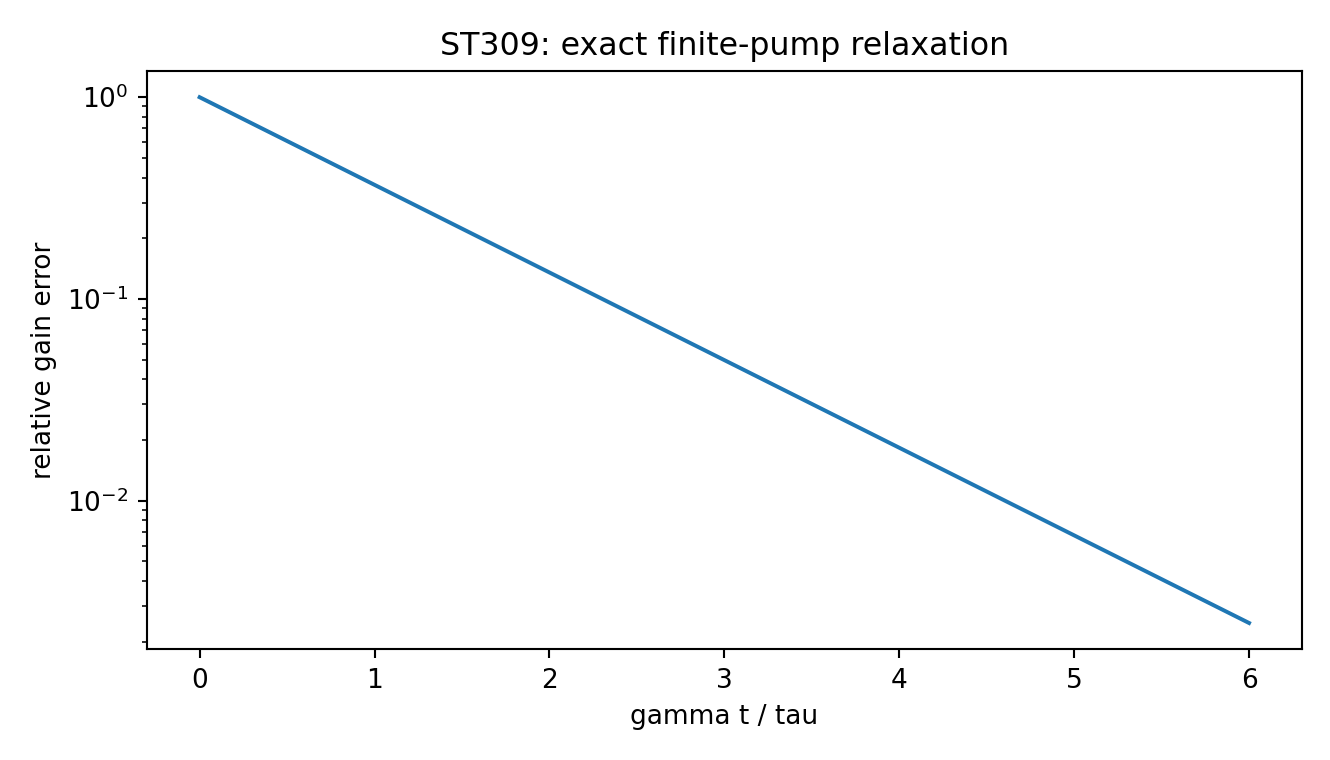
\includegraphics[width=.72\textwidth]{FIN_ST308_ST326_Figures/st309_pump_relaxation.png}
\caption{Exact relaxation of a finite pumped auxiliary. The horizontal variable is dimensionless; no physical pump has been identified.}
\end{figure}

The more important correction is that a pump is not logically necessary for a static
negative Schur term. For a positive conservative mediator,
\[
\mathcal E(q,y)=\frac12\langle y,\Gamma y\rangle-\langle y,Bq\rangle,
\qquad \Gamma\succ0,
\]
elimination gives
\[
\inf_y\mathcal E(q,y)=-\frac12\langle q,B^T\Gamma^{-1}Bq\rangle .
\]

\begin{theorem}[minimal linear mediator rank]
If $B^T\Gamma^{-1}B=gA$, then $\dim y\ge\operatorname{rank}A=11$.
Conversely $11$ dimensions attain equality by taking $B=\sqrt g\,A^{1/2}$ on
$\operatorname{ran}A$.
\end{theorem}

Thus the honest trichotomy is: passive dissipative memory cannot deliver gain; a pumped
auxiliary can; a conservative mediator can generate the static negative term without a
pump. Both successful mechanisms add signed coupling data. After loss of quadratic
stability, either also needs a stabilizing nonlinear sector. None sources $g$ from the
present strict kernel.

\section{ST311--ST313: certified localization and the global question}

At $g=4$ the reflection-even stationarity equations are
\[
\log(12q_i)+1-4(Bq)_i+\lambda=0,\qquad
q_0+2\sum_{i=1}^5q_i+q_6=1,
\]
where $B$ is the seven-orbit radial compression of $A$. An outward Krawczyk box of radius
$10^{-8}$ has inclusion margin $9.9866\times10^{-9}$. Its probability lower bound is
positive. A sum-zero tangent congruence for
\[
\operatorname{diag}(1/p)-4A
\]
has a conservative perturbation-paid lower bound $83.76>0$.

\begin{theorem}[localized orbit at supplied gain]
For every strict operator in the declared transcendental interval family, there is one
strict reflection-even local minimum in the accepted box at $g=4$. Its twelve cyclic
translations are distinct strict local minima.
\end{theorem}

The certified value is approximately $-0.84519851$, lower than the uniform value $0$ and
the pure-vertex value $-0.83570791$. This is a local existence theorem, not proof that
there are exactly twelve critical points or that these are global vacua.

ST312 supplies an exact smaller global target. Fenchel completion gives
\[
\inf_{h\perp\mathbf1}\left\{
\frac{1}{2g}\langle h,A^+h\rangle-\log\!\left(\frac1{12}\sum_i e^{h_i}\right)
\right\},
\]
with fixed point $p_i\propto e^{g(Ap)_i}$. Three hundred frozen starts find no value below
the certified branch, but the resulting 11-dimensional nonconvex problem has not been
interval-covered. Globality remains open.

\begin{figure}[H]\centering
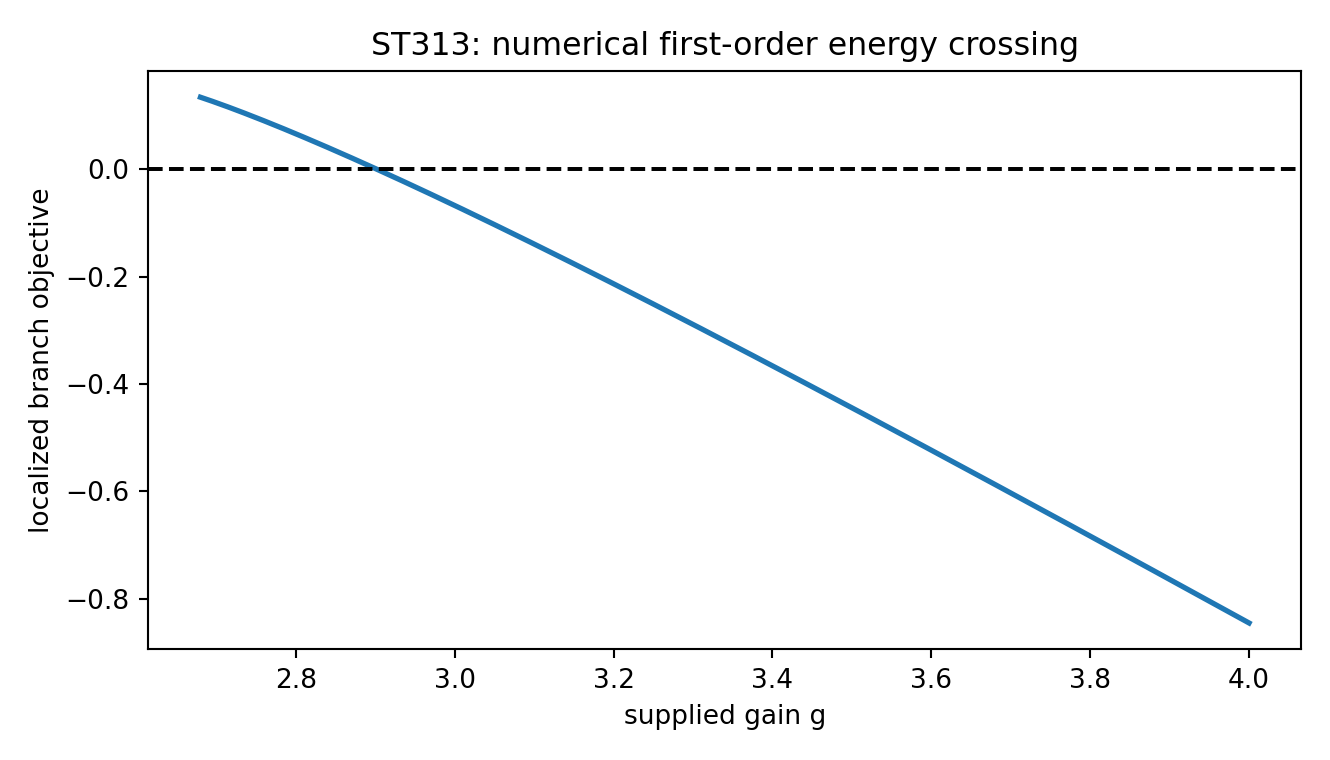
\includegraphics[width=.76\textwidth]{FIN_ST308_ST326_Figures/st313_branch_crossing.png}
\caption{Numerical continuation of the localized stationary family. The energy crossing is evidence, not an interval transition theorem.}
\end{figure}

The sampled branch remains regular and crosses uniform energy in
$g\in[2.900,2.905]$, below the vertex comparison $g_E\approx2.99331$ and far below the
uniform Hessian instability $g_{\rm Hess}\approx5.12343$. This strengthens the first-order
transition picture but does not certify the crossing or spinodal.

\section{ST314--ST318: completion of four mathematical frontiers}

The 160 ST298 boxes are separated: the smallest center distance after paying both radii is
$2.496\times10^{-5}>0$. They certify discrete pseudo-arclength sections, not a connected
tube. Of 20 representative half-step enclosures, only 13 pass. This is an explicit gap in
the old inference, not evidence that the smooth branch itself breaks.

ST315 closes one three-output SDP exactly. For
\[
\tau_0=\begin{pmatrix}3/4&0\\0&1/4\end{pmatrix},\quad
\tau_{\pm}=\begin{pmatrix}1/2&\pm1/4\\\pm1/4&1/2\end{pmatrix},
\]
the dual $\Gamma=3I/4$ and POVM $(0,|+\rangle\langle+|,|-\rangle\langle-|)$ are feasible
with the same exact value $3/2$. Weak duality proves global optimality. The first output is
ignored, illustrating why a single binary positive-part rule is not a multi-output formula.

ST316 pays the missing filter contraction. Every frozen positive two-state HMM matrix has
cross ratio $36$, hence Birkhoff coefficient
\[
\tanh\!\left(\frac14\log36\right)=\frac57.
\]
This controls belief forgetting but does not yet control the entire normalized Chernoff
derivative operator; the infinite-depth optimizer is still not certified.

ST317 proves a general allocation rule. Under a product budget and linearized loads
$a_i/n_i$, minimax allocation has $n_i\propto a_i$. The numerical FIN sensitivities suggest
integer counts $(41,25,62)$, using 63,550 cells. This is a design predictor, not a complete
outward cover.

ST318 substantially strengthens the old determinant no-go.
\begin{theorem}[sharp odd-dimensional approximation obstruction]
If $X,Z$ are Hermitian involutions in odd complex dimension, then
\[
\|XZ+ZX\|_{\rm op}\ge2.
\]
The bound is sharp.
\end{theorem}
Indeed $U=XZ$ is unitary and $XUX=U^*$, so nonreal eigenvalues pair by conjugation. Odd
dimension leaves an eigenvalue $\pm1$, on which $U+U^*$ equals $\pm2$. Exact involutions
cannot approximate anticommutation below a fixed error in odd dimension.

\section{ST319--ST321: scale cocycles, infrared design, and anchors}

The internal-observer note proposed a calibration bundle over refinements. ST319 identifies
its first obstruction. On a tree, choose a root and define $h_n$ as the product of edge
calibrations along the unique path. Every positive cocycle is then
\[
g_{mn}=h_m/h_n.
\]
It is a coboundary. A nonconstant vertical rate is therefore pure calibration gauge on a
tree; observable holonomy requires cycles, and an absolute magnitude requires an anchor.

ST320 replaces the ST304 smooth-family grid by a pointwise theorem. For measurable
$0\le q(\mu)\le1$ and one heat budget, maximizing a single-time dimension functional is a
bathtub problem ordered by
\[
\frac{4\mu t/(e^{2\mu t}+1)}{e^{-2\mu t_0}}.
\]
The unrestricted extremizer is bang--bang up to one threshold level set. Smooth near-Haar
profiles may be better for a time-window minimax objective, but they are not pointwise
extremizers. The minimax plateau problem remains open.

The original calibration group has coordinates $(L,T,E)$ and dimension three. If physics
supplies both a speed relation $L/T$ and an action relation $ET$, their exponent rows have
rank two. The residual scaling is
\[
(\ell,\tau,\varepsilon)\mapsto(a\ell,a\tau,\varepsilon/a).
\]
One independent dimensional anchor remains necessary. This reduces Bridge U; it does not
derive $c$, $\hbar$, their numerical values, or their identification with FIN channels.

\section{ST323--ST326: operational layer depth and controlled fractal compression}

The most valuable unused suggestion from the internal-observer note was to define a layer
by its available experiment rather than by a pictorial depth index. For
\[
\widetilde A=RAR^*\oplus B,
\]
coarse preparations and effects supported in $\operatorname{ran}R$ are independent of $B$.

\begin{theorem}[observer blindness kernel]
For a two-child 12-dimensional fiber, arbitrary symmetric $\delta B$ form a
78-dimensional blindness kernel for the coarse context. If ideal fiber-complete records
contain $e^{-tB}$ on an open time interval, differentiation at $t=0$ recovers $B$ and the
kernel is zero.
\end{theorem}

Blackwell dominance gives a sound depth preorder: if every coarse record is a stochastic
postprocessing of fine records, then
\[
\mathcal N_{\rm fine}\subseteq\mathcal N_{\rm coarse}.
\]
The converse is false. Binary symmetric channels with error $0.1$ and $0.2$ both identify
their scalar input parameter and thus have zero kernel, while the latter is a strict
garbling of the former. Kernel dimension alone is too crude; the experiment category must
be retained.

Exact intertwining transports each coarse mode with the same eigenvalue. Therefore
unitary phase-frequency ratios and heat-rate ratios $\lambda_i/\lambda_j$ are exactly
refinement-natural, while wave-frequency ratios are
$\sqrt{\lambda_i/\lambda_j}$. Fiber clocks depend on free $B$. Relative cycles survive;
seconds, a time arrow, and inter-fiber comparison do not emerge.

Finally, the controlled meaning of ``fractal information compression'' is limited by
counting. If every layer has $b$ arbitrary branch choices, a lossless record of depth $n$
has $b^n$ possibilities and needs at least
\[
n\log_2 b
\]
bits. A finite kernel may compress the repeated rule. It cannot losslessly store every
arbitrary history with bounded extra data. Stronger compression requires a restricted
state class, correlations, or loss, together with an encoder, decoder, and distortion
bound.

\section{What from the two suggestion maps remains worth studying?}

\begin{longtable}{p{.25\textwidth}p{.24\textwidth}p{.43\textwidth}}
\toprule Suggestion&Current verdict&Next legitimate move\\\midrule\endhead
Layer as available operations&Substantially advanced by ST323--ST324&Classify intermediate, noisy instrument families and quantitative deficiency, not only ideal endpoints.\\
Calibration bundle and cocycle&Tree cocycles are gauge-trivial; two supplied relations leave one orbit&Study cyclic refinement categories and whether any strict observable creates nontrivial holonomy.\\
Internal clock&Coarse ratios are natural; absolute time and arrow remain absent&Construct a record-bearing oriented clock only with a genuinely new non-premise source; do not replay QW-2191.\\
Observer-specific plateau&Single-time extremizer is bang--bang; minimax window open&Prove a multi-time bathtub/duality theorem with an explicit observer response kernel.\\
Fractal compression&Rule compression survives; arbitrary histories need linear record growth&Define a FIN state class and rate--distortion problem; test whether strict refinement gives useful correlations.\\
Sourced phase state&Local minima now certified at supplied $g$; source and globality open&Certify the crossing/spinodal and globally cover the 11-dimensional dual; separately derive or axiomatize the signed coupling.\\
Physical projection&Still a counterfactual H\_PROJ&Wait for a typed apparatus and independent records; local code cannot upgrade it.\\
Absolute Planck/SI scale&Obstructed from invariant dimensionless data&Do not revisit without a new dimensional source or an explicitly supplied anchor.\\
\bottomrule
\end{longtable}

The audit therefore validates the relational and operational parts of the AI suggestions,
while rejecting their possible promotion to ``our layer generates metres,'' ``the universe
is a projection,'' or ``fractal compression stores all histories for free.''

\section{Falsification ledger and surviving interpretation}
\begin{longtable}{p{.27\textwidth}p{.29\textwidth}p{.37\textwidth}}
\toprule Claim&Test&Surviving statement\\\midrule\endhead
Active gain necessarily requires a pump&Positive mediator elimination&False: a conservative Schur mediator also works, but imports signed coupling and at least 11 states for full $A$.\\
$g=4$ localization is only numerical&Outward root and Hessian bounds&False locally: twelve translated strict local minima are proved. Globality remains open.\\
The localized orbit is globally proved&Exact dual plus multistart&False: the dual remains an uncovered 11-dimensional problem.\\
ST298 boxes make a tube&Box-distance audit&False: accepted boxes are disjoint.\\
Three-output recovery lacks an exact case&Rational primal-dual witnesses&False: the displayed fixture has optimum $3/2$.\\
Odd Clifford pairs can become arbitrarily good&Unitary conjugate-pair argument&False for exact involutions: error is at least $2$.\\
A nonconstant scale law is observable on a hierarchy&Tree cocycle classification&False on a tree without anchors or cycles; it is gauge.\\
Blindness-kernel dimension fully orders observers&Blackwell counterexample&False; experiment postprocessing contains more information.\\
Fractal self-similarity stores arbitrary histories at fixed cost&Counting bound&False losslessly; the rule is short but arbitrary records grow linearly in depth.\\
Local output is experiment&Independent-record search&False; ST322 is blocked.\\
\bottomrule
\end{longtable}

The deepest interpretation surviving this batch is:
\begin{quote}
The strict FIN operator supplies a symmetric relational carrier and a family of response
channels. A localized information phase is mathematically real once a sufficiently strong
signed interaction is supplied, but neither its coupling nor its global physical selection
is yet strict-derived. Refinement does not create an absolute scale; it creates an
experiment-dependent hierarchy of distinguishability, natural relative clocks, and a
calibration gauge. Fractal compression belongs to the law of repetition, while histories,
anchors, and records remain resources. The missing physics is therefore a sourced signed
interaction, a globally controlled phase law, an operational apparatus with anchors, and
independent events---not another reinterpretation of the spectrum.
\end{quote}

\section{Recommended programs ST327--ST341}
\begin{enumerate}
\item[\textbf{ST327}.] Interval-certify the localized energy crossing by two Krawczyk root
boxes plus an interval sign proof for $V_g$.
\item[\textbf{ST328}.] Continue to and certify the localized spinodal with validated
pseudo-arclength and a simple-nullity theorem.
\item[\textbf{ST329}.] Build a complete interval branch-and-bound for the exact ST312 dual,
or return a frozen-resource no-go with uncovered boxes recorded.
\item[\textbf{ST330}.] Classify $D_{12}$-covariant conservative mediators of dimension
$m<11$ and quantify their best spectral approximation to $gA$.
\item[\textbf{ST331}.] Test whether an existing strict nonlinear invariant can stabilize
the Schur-mediated phase without importing a branch or selector.
\item[\textbf{ST332}.] Derive a weighted derivative-tail bound from the exact $5/7$
projective contraction, or exhibit the missing noncontractive weight mode.
\item[\textbf{ST333}.] Replace the disjoint ST298 boxes by an interval implicit-function
cover with overlapping parameter slabs; stop at the first certified obstruction.
\item[\textbf{ST334}.] Solve the multi-time soft-IR minimax problem by convex duality and
identify whether extremizers require finitely many threshold bands.
\item[\textbf{ST335}.] Classify scale-cocycle holonomy on the smallest refinement diagram
with a genuine cycle; separate gauge invariants from path artifacts.
\item[\textbf{ST336}.] Construct quantitative observer depth using Le Cam deficiency for
coarse, partially child-resolving, and fiber-complete instruments.
\item[\textbf{ST337}.] Add finite-count noise to ST323 and derive a minimax lower bound for
recovering $B$ from child-resolved heat records.
\item[\textbf{ST338}.] Formulate the FIN refinement state class and compute a first
rate--distortion bound; no universal compression claim without it.
\item[\textbf{ST339}.] Test relative-clock consistency when coarse modes mix with fiber
modes under approximate rather than exact intertwining.
\item[\textbf{ST340}.] Audit every proposed cross-channel relation by dimensions and
identifiability before using it to reduce the calibration group.
\item[\textbf{ST341}.] Resume empirical work only after provider--registrar--analyst
separation and independently hashed raw events exist.
\end{enumerate}

The highest mathematical priorities are ST327 and ST329: they decide whether the newly
certified local phase can become a global theorem. ST330--ST331 address the strict source
gap without silently importing a pump. The most valuable continuation of the user's layer
intuition is ST336, because it turns ``seeing through fractal layers'' into a quantitative
comparison of experiments rather than a visual metaphor.

\section{Reproducibility and conclusion}

The source \texttt{fin\_st308\_st326\_research.py} writes nineteen individual packets, an
aggregate JSON, a CSV ledger, and two figures. The independent suite
\texttt{test\_fin\_st308\_st326.py} performs twenty live tests covering packet hashes,
thresholds, exact auxiliary relaxation, mediator rank and reconstruction, live localized
stationarity, interval/Hessian flags, energy ordering, crossing signs, tube gaps, the exact
SDP, Birkhoff contraction, allocation budget, the sharp Clifford bound, cocycle
reconstruction, calibration rank, empirical stop, blindness dimensions, Blackwell
garbling, refinement intertwining, and the compression count. All twenty tests pass.

This batch advances two bridges and narrows a third. The state bridge now has a proved
localized phase at supplied gain. The observer bridge now has an exact blindness kernel,
a sound depth preorder, and refinement-natural relative clocks. The unit bridge is reduced
to one orbit only after two physical relations are supplied. The central source gap remains:
present strict FIN does not select the signed interaction, stabilizer, calibration anchors,
or empirical realization. Those boundaries are now explicit mathematical objects rather
than philosophical omissions.

\end{document}
